\section{Methodology} \label{sec:methodology}

In this chapter, we describe methods and principles applied in the course of this project. We begin with elucidation of the development process, model applied and structure of the work. Difference between the minimum viable product and prototype are laid down and the purpose and need of use cases and requirements is shown. Lastly main \acrshort{uml} diagrams used are explained.

\subsection{Software Development Process}

The development process describes the organisation and grouping of activities during the life-cycle of a given system. The basic activities of software development are:
% 
\begin{enumerate*}[label=(\roman*)]
    \item requirement elicitation,
    \item design,
    \item implementation,
    \item testing,
    \item integration, and
    \item maintenance~\cite{Sommerville2011SoftwareEngineering, CMS2005SELECTINGAPPROACH}.
\end{enumerate*}
% 
Software development process organises these components in the most optimal way to produce high quality software at lowest possible cost. Because every development project varies in scope, resources and desired outcome, the software development process needs to be adjusted for each project individually to best meet the needs of that project. While there is no single correct way to organise the software development process, two most prominent models can be identified -- waterfall, and agile~\cite{Sommerville2011SoftwareEngineering}.

In a waterfall model, the basic activities are carried out in a sequential fashion. Once an activity is completed, it's outputs are determined, ``signed-off'', and are not modified further in the process, This mandates that the requirements are fully specified, before the work on system design commences; the system design needs to be completed, before implementation can begin, and so on. True waterfall is rarely used in practice, since requirements tend to change as the development progresses and implementation needs to be changed as errors are discovered during testing.

There are several different methodologies which may be loosely grouped under the \textit{Agile} category (Scrum, Kanban, Lean development and other), however they are based on a common set of principles based on welcoming (and even embracing) the changes to scope and requirements throughout the development process~\cite{KentBeck2001ManifestoDevelopment}. This is reflected by iterative and incremental development, where the activities are often revisited as the development progresses and the software is built and released in parts -- increments, where each new release carries more functionality that the previous release. The agile development is widely used in practice and organisations which previously followed the waterfall model are transitioning to agile more often, than the other way round~\cite{Sommerville2011SoftwareEngineering}.

This project follows a modified waterfall model. As this is a research project, focus is put on innovation and utilisation of new technologies, over delivery and integration of a stable, production-grade software. The project progresses through the following stages:
% 
\begin{enumerate*}[label=(\roman*)]
    \item Initial Research,
    \item Requirement Elicitation,
    \item Design,
    \item Implementation, and
    \item Testing \& Evaluation, in this order. 
\end{enumerate*}
% 
The progress is not iterative, once a stage is completed, the outcomes are written down, documented and used as inputs to the next stage. Main reason for this approach is the relative short duration of the project, that do not allow for completion of more than 2-3 iterations. Another reason is, that while agile methodologies cater to changing customer requirements, the customers' demands in this project are assumed and theorised and do not change significantly through the course of the development. Finally, there is no ask to release the software in increments. Longer planning phase and a single implementation phase help to avoid the complexity, which arises from iterative organisation of the work. Figure~\ref{fig:development-process} illustrates the development process used in this project.

\begin{figure}[htpb]
    \centering
    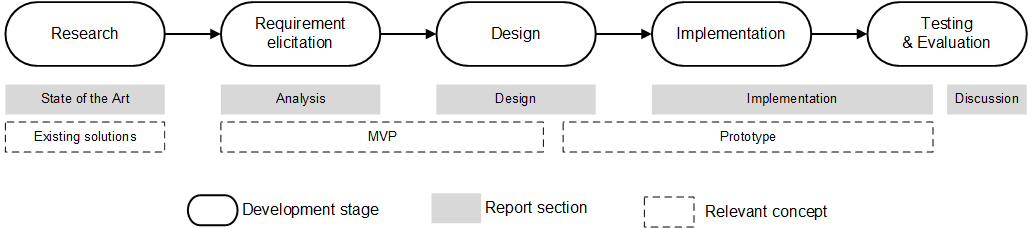
\includegraphics[width=\textwidth]{development-process}
    \caption{The modified waterfall model used in this project (rounded boxes). Below, the corresponding report chapters are shown (grey boxes) and relevant scopes for that stage (dashed boxes).}
    \label{fig:development-process}
\end{figure}

The \textit{initial research} stage is not typically mentioned as a separate stage in literature~\cite{Sommerville2011SoftwareEngineering, CMS2005SELECTINGAPPROACH}, however we list is here separately, as exploring the state-of-the-art technologies and solutions is necessary in a research project. In the requirement elicitation and design, an~\acrfull{mvp} is considered (elaborated on in the following section). From the outputs the design stage, a set of few use-cases is selected, which are then implemented in a prototype
 (the prototype is discussed in section \ref{sec:methodology-prototype}). Integration and maintenance stages are omitted this project, as the goal is not to produce and deploy the software into production.
\subsection{Minimum Viable Product}
The \acrfull{mvp} is described as the minimal set of features that a customer would be willing to pay for~\cite{SteveBlank2010PerfectionFeatureSet}. It does not describe a desired final state of the product, rather it describes a first marketable version. The first version is only aimed at a fraction of the market, at customers known as \textit{early adopters}, who are more forgiving towards lower utility and are more likely to provide early feedback on the product. If any one feature would be removed from the \acrshort{mvp}, the product would have such a limited utility, that it would be very unlikely adopted by any customers, even the early adopters~\cite{Junk2000TheProjects}.

While this project does not examine the market for this solution, we use the \acrshort{mvp} methodology to focus on most important product features in the requirement elicitation and design stages. The \acrshort{mvp} approach helps us identify, which features need to be present in the prototype and the first version of the product, and to differentiate the product developed in this project from the full-featured product, which would be achieved if the project continued further.
\subsection{Software Prototyping}\label{sec:methodology-prototype}

A prototype is a model, an initial version of the intended system. The goal of the prototype is to demonstrate the final product, present the idea, test out design choices or compare two variants of the product. It is cheaper and faster to produce a prototype than it is to produce a fully functional system, so the prototype can also be used to reduce risk from uncertain requirements~\cite{Sommerville2011SoftwareEngineering, Davis1995SoftwarePrototyping}.

It is argued, that the purpose of the prototype needs to be determined early for the prototype to bring value and that the prototype must be evaluated after it is implemented. In this project, the prototype is implemented to demonstrate the feasibility of the technology in the access control scenario. It achieved by implementing a subset of the requirements in an experiment prototype. Experiment prototype verifies a possible solution to user needs, but leaves out the user interface choices and non-functional requirements (such as speed or reliability). This is contrasted by exploratory prototype (used to discover new requirements) and evolution prototype (prototype that is iteratively evolved into the final product)~\cite{Davis1995SoftwarePrototyping}.
\subsection{Use Cases}
Use case \textit{``represents the list of tasks that actors can perform, and is directly related to the requirements''}~\cite{IBMKnowledgeCenter2019DefiningCases}Defining use cases. It depicts functionality of the system in the context of the use by the actor who is interacting with it. List of requirements can be subsequently extracted from use cases. To describe possible use of the system, a set of use cases is created which will serve as a base for the requirements specification.
\subsection{Requirements}
System Requirements specification is \textit{``a structured collection of information that embodies the requirements of the system''}~\cite{ISO2010ISO/IEC/Vocabulary}. There are two types  of requirements: 
\begin{itemize}[noitemsep]
    \item Functional requirements - \textit{``specifies a function that a system or system component must be able
to perform''}~\cite{ISO2010ISO/IEC/Vocabulary}
    \item Non-functional requirements - \textit{``a software requirement that describes not what the software will do, but how the software will do it''}~\cite{ISO2010ISO/IEC/Vocabulary}.
\end{itemize}

By specifying system requirements, both functional and non-functional ones, we are able to define system's functionality and performance metrics, so when system design phase begins, it is clear what a system must fulfil in order to perform reliably and satisfactory.  

\subsection{Unified Modeling Language}
\acrfull{uml} is \textit{``A specification defining a graphical language for visualising, specifying, constructing, and documenting the artifacts of distributed object systems.''}~\cite{OMG2017About2.5.1}. The latest version of the specification is \acrshort{uml} 2.5.1 which was published in 2017. It is describes a set of diagrams and their standardised notations, which are used in software system and business modelling, as well as other non-software modelling tasks. In total 14 \acrshort{uml} diagrams are defined. There are two principal types of diagrams: \textit{Behaviour} and \textit{Structure} diagrams~\cite{ObjectManagementGroup2015Unified2.5}. Main difference between the two is that Behaviour diagrams indicate system's objects dynamic behaviour and Structure diagrams indicate their static structure. In this project, we have use one structure diagram -- a class diagram and two behaviour diagrams -- use case and sequence diagrams, which help us to visualise flows in the system and document the implemented prototype.

\subsubsection{Class diagram}
Class diagram is a static diagram which specifies the structure of the system. It is used for detailed modelling of the application's structure by visualising all classes, containing the name, attributes and operations of the class, and static relationships between them. Detailed and well designed class diagram can afterwards be translated to a programming code. Designing a class diagram before programming can help to structure the code better and save time during the programming phase. The class diagram can also be used to document the existing code~\cite{Seidl2015UMLModeling}.

\subsubsection{Use case diagram}
Use case diagram is a behaviour diagram which describes the interaction of an external user with a system. Main components of a use case diagram are use cases, actors, associations. Actors are external users, humans or other systems, who are interacting with the system. Actors may proactively request services from the system, or may react to requests made by the system~\cite[p.~28]{Cockburn2000WritingCases}. Use cases depict a possible scenarios and use of a system which an actor can come across and are drawn in ovals. Associations are relations between use cases and actors. Use case diagram helps us to visualise all actors of our system, both humans and external systems, to know and see with which use cases are they interacting with, and where are the boundaries of our system.

\subsubsection{Sequence diagram}
Sequence diagram is a behaviour diagram describing the interaction between objects and their message exchange in sequence. It consists of vertical lines known as lifelines which represent objects and processes that run in parallel, and horizontal lines which represents messages that are being interchanged in sequence. We use the sequence diagram to demonstrate message exchange between entities of our system in a few basic scenarios.

\bigskip\noindent
The above mentioned methods and principles allow us to carry out the work on the project in a systematic and structured way while following the standardised industry approaches, which guarantee that everyone who knows the standard can understand the work carried out.